\documentclass[border=4pt]{standalone}
\usepackage[T1]{fontenc}
\usepackage{helvet}
\renewcommand{\familydefault}{\sfdefault}
\usepackage{graphicx}
\usepackage{caption}
\usepackage{amsmath}
\captionsetup{font={sf,footnotesize},labelfont={sf,bf,footnotesize},justification=justified,singlelinecheck=false}
\begin{document}
\setcounter{figure}{14}
\begin{minipage}{7.20in}
\centering
\begin{figure}[htbp]
    \centering
    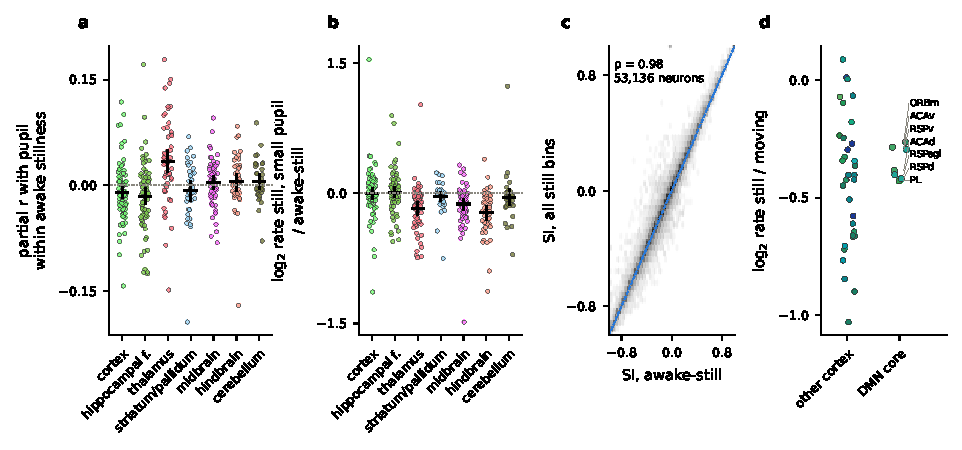
\includegraphics[width=\linewidth]{fig15_still_arousal_panels.pdf}
    \caption{Arousal within stillness, the sleep gate and the DMN core. \textbf{a} Partial correlation of each neuron's 1\,s spike count with pupil diameter within awake stillness (time and motion energy regressed out); dots are mice. \textbf{b} Rate in still bins with a pupil below the gate (but $\leq$30\,s since movement) relative to awake stillness; lower in thalamus, midbrain and hindbrain, unchanged in cortex and hippocampus. \textbf{c} Stillness index with and without the anti-sleep gate. \textbf{d} Cortical regions: conservative DMN core vs other cortex (core -0.35, other -0.43, region permutation p = 0.49); dots in Allen atlas region colours.}
    \label{fig:arousal}
\end{figure}
\end{minipage}
\end{document}
